\section{Density Functional Formalism}
Modern first-principles electronic strucutre calculations in solids are always based on the density functional therem (DFT) of P. Hohenberg and W. Kohn (1964)~\cite{hohenberg1964inhomogeneous}. It states that the Total Energy, $E$, of a non-spin-polarized system of interacting electrons in an external potential (i.e Coulomb potential due to the nuclei in a solid) is exactly a functional of the ground state electronic density, $\rho$.
\begin{equation}
E = E[\rho]
\end{equation}
It also showed that the true ground state density is the desnity that minimizes $E[\rho]$, and the other ground state properties are also functionals of the ground state. Before Hohenberg and Kohn, the original density functional theory of quantum system is the method of Thomas~\cite{thomas1927calculation} and Fermi~\cite{fermi1927metodo} proposed individually in 1927. In the Thomas-Fermi method the Kinetic energy of the system electrons is approximated as an explicit functional of the density. This model fails to explain some of the useful description of the electrons in matter.

Even though original paper only talked about non-spin-polarized system, the extension to spin-polarized systems is straightforward. The E and other ground state properties become functionals of the spin density. In a simple collinear case, where the spin-up and spin-down densities are enough, then the ground state would be :
\begin{equation}
	E =E[\rho_{\uparrow},\rho_{\downarrow}]
\end{equation} 
The H-K theorem does not provide any guidance how to achieve $E[\rho]$, and the usefulness of DFT depends on the proper approximation of the functional. To approach this challenge, the unknown functional, $E[\rho]$, is written as the Hartree total energy plus another, but presumably smaller, unknown functional, called the exchange-correlation (xc) functional, $E_{xc}[\rho]$.
\begin{equation}
\label{eq_main_func}
E[\rho] = T_s[\rho] + E_{ei} [\rho] + E_H[\rho] + E_{ii}[\rho] + E_{xc}[\rho]
\end{equation}
Here $T_s{\rho}$ denotes the single particle kinetic energy, $E_{ei}[\rho]$ is the Coulomb interaction energy between the electrons and the nuclei, $E_{ii}[\rho]$ arises from the interaction between the nuclei with each other, and $E_H[\rho]$ is Hartree component of the electron-electron energy,
\begin{equation}
\label{eq_hartree}
E_H[\rho] = \frac{e^2}{2}\int d^3\mathbf{r}d^3\mathbf{r'} \frac{\rho(\mathbf{r})\rho(\mathbf{r'})}{\abs{\mathbf{r}-\mathbf{r'}}}
\end{equation}
$E_{xc}[\rho]$ is an unknown functional. Nonetheless, several useful approximations to it are known. The simplest is the local density approximation (LDA). In the LDA, $E_{xc}[\rho]$ is written as
\begin{equation}
E_{xc}[\rho] = \int d^3\rho(\mathbf{r})\epsilon_{xc}(\rho(\mathbf{r}))
\end{equation}
Where $\epsilon_[xc]$ is approximated by a local function of the density, usually that which reproduces the known energy of the uniform electron gas. The other commonly used approximations are the generalized gradient approximations (GGAs), where the local gradient as well as the density is used in order to incorporate more information about the electron gas ( $\epsilon_{xc} (\rho)$ is replaced by $\epsilon_{xc}(\rho,\abs{\nabla\rho)}$. The relation between the different approximations can be understood using the exact expression for the exchange correlation energy in terms of pair correlation function~\cite{langreth1975exchange}.

Kohn and Sham~\cite{kohn1965self} wrote the electron density as a sum of single particle densities, and used the variational property to find a way to calculate the ground state energy and density, given the functional $E_{xc}$. More precisely, they showed that the correct density is given by the self-consistent solution of a set of single particle \schrod-like equations, known as Kohn-Sham (KS) equation, with a dependent potential,
\begin{equation}
\label{eq_ks}
\{T + V_{ei}(\mathbf{r}) + V_H (\mathbf{r}) + V_{xc}(\mathbf{r})\}\varphi_i(\mathbf{r}) = \epsilon_i \varphi_i(\mathbf{r})
\end{equation}
Where the density is given by a Fermi sum over the occupied orbitals,
\begin{equation}
\label{eq_ks_orbit}
\rho(\mathbf{r}) = \sum_{occ} \varphi^{\ast}_i (\mathbf{r})\varphi_i(\mathbf{r})
\end{equation}
Here the highest occupied orbital is determined by the electron count, the $\varphi_i$ are the single particle K-S orbitals, the $\epsilon_i$ are the corresponding K-S eigenvalues, $T$ is the single particel kinetic energy operator, $V_{ie}$ is the Coulomb potential due to the nuclei, $V_H$ is the Hartree potential and $V_{xc}$ is the exchange correlation potential. Both $V_{xc}$ and $V_H$ depend on $\rho$.
\begin{equation}
\label{eq_hartree_density}
V_H(\mathbf{r}) = e^2 \int d^3 \mathbf{r}' \frac{\rho(\mathbf{r'})}{\abs{\mathbf{r}-\mathbf{r'}}}
\end{equation}

\begin{equation}
\label{eq_xc_ks}
V_{xc}(\mathbf{r}) = \frac{\delta E_{xc}[\rho]}{\delta\rho(\mathbf{r})}
\end{equation}
In this framework, a calculation entails the self-consistent solutions of Eqn~\ref{eq_ks} and \ref{eq_ks_orbit}. Which usually means, a density must be found such that it yields an effective potential that when inserted into the \schrod-like equations yields orbitals that reproduces it. In this way, instead of solving a many-body \schrod equation using DFT,  the problem is now solving a series of single particle equations, with the requirement of self-consistency. This leads to a wide variety of technique regarding DFT. The plane-wave expansion of K-S orbitals are widely used in codes like QuantumEspresso and Abinit. The method to use a basis to represent the KS orbitals are:
\begin{equation}
\label{eq_basis}
\varphi_i (\mathbf{r}) = \sum_{\alpha} c_{i\alpha} \phi_{\alpha} (\mathbf{r})
\end{equation}
Where the $\phi_{\alpha}(\mathbf{r})$ are the basis functions and the $C_{i\alpha}$ are expansion coefficients.

\subsection{Solution of the Single particle Kohn-Sham Equations}
The previous chapter addressed the formation of K-S equation and the idea of self-consistency. In DFT based calculation, methods are classified based on the representation of the density, potential and especially KS orbitals. The choice of representation is made to increase the computational efficiency, while maintaining the accuracy.
For a choice of basis, the coefficients are the only variable to be determined (density depends on KS orbitals). The total energy of DFT becomes variational, then the solution of the self-consistent KS equations requires to determine the $C_{i\alpha}$ for the occupied orbitals that provides a minima of the total energy.

According to the second theorem of Hohenberg and Kohn, all properties such as kinetic energy, etc. are uniquely determined if $\rho(\mathbf{r})$ is specified. Eqn~\ref{eq_ks} shows the relationship. To minimize the total energy with respect of KS orbitals, the variational principle is usually used. While performing the minimization, it is prefer to minimize with $\varphi^{\ast}(\mathbf{r})$ (both yield the same result). Using the chain rule for functional derivatives, the equations becomes:
\begin{equation}
\label{eq_var_ks}
\frac{\delta E}{\delta \varphi^{\ast}_i(\mathbf{r})} = \frac{\delta T_s}{\delta \varphi^{\ast}_i(\mathbf{r})} + \left [ \frac{\delta E_{ext}}{\delta \varphi^{\ast}_i(\mathbf{r})} + \frac{\delta E_H}{\delta \varphi^{\ast}_i(\mathbf{r})} + \frac{E_{xc}}{\delta \varphi^{\ast}_i(\mathbf{r})}	\right ] \frac{\delta \rho(\mathbf{r})}{\delta \varphi^{\ast}_i(\mathbf{r})}  = 0
\end{equation}
The kinetic energy may be differentiated separated with respect to orbital. In the above equation the $E_{ei}$ is replaced with $E_{ext}$ which means potential due to nuclei and any other external fields\footnote{Deriving Eqn~\ref{eq_var_ks_eig} from Eqn~\ref{eq_var_ks} involves variational principle with Lagrange multiplier.}.
\begin{equation}
\label{eq_var_ks_eig}
-\frac{1}{2} \nabla^2 \varphi^{\ast}_i (\mathbf{r}) + \left [ V_{ext} (\mathbf{r}) + \int d(\mathbf{r'}) \frac{\rho(\mathbf{r'})}{\abs{\mathbf{r}-\mathbf{r'}}} + \epsilon_{xc} (\rho) + \rho(\mathbf{r}) \frac{\delta \epsilon_{xc}[\rho]}{\delta \rho(\mathbf{r})}   \right ] \varphi_i(\mathbf{r})  = \epsilon_i \varphi_i (\mathbf{r})
\end{equation}
Eqn~\ref{eq_var_ks_eig} is a system of equations, represent the many-particle system in terms of single-particle orbitals. Each of these equations resemble a \schrod equation
\begin{equation}
\label{eq_ks_s}
\left [ \hat{T} + V_{eff}\right ] \varphi_i (\mathbf{r}) = \epsilon_i \varphi_i (\mathbf{r})
\end{equation}

Deriving Eqn~\ref{eq_var_ks_eig} from Eqn~\ref{eq_var_ks} involves variational principle and using Lagrange multiplier for \schrod equation. Here the $V_{eff}$ is the sum of the $V_H$, $V_{xc}$ and $V_{ext}$, which depends on the density and indirectly depends on orbitals. Now we have an equation where any change in the orbitals effect also the potential on which they in turn depend on orbital. This problem is resolved by solving Kohn-Sham system of equations self-consistently.
\begin{center}
\begin{figure}
\begin{tikzpicture}[node distance =2 cm, auto]
	\node [block] (inguess) {Initial guess};	
	\node [block] (inguess2) [below of =inguess, yshift=0.75 cm] {$\rho(\mathbf{r})$};
	\node [block2] (cal1) [below of = inguess2] {Calculate effective potential};
	\node [block2] (cal2) [below of =cal1, yshift = 0.75 cm] {$V_{eff}(\mathbf{r}) = V_{ext} (\mathbf{r}) + V_H[\rho] + V_{xc} [\rho]$};
	\node [block2] (sol1) [below of = cal2] {Solve KS equations};
	\node [block2] (sol2) [below of = sol1, yshift = 0.75 cm] {$\left [-\frac{1}{2} \nabla^2 + V_{eff}(\mathbf{r}) \right] \varphi_i(\mathbf{r}) = \epsilon_i \varphi_i(\mathbf{r})$};

	\node [block2] (den1) [below of = sol2] {Calculate electron density};
	\node [block2] (den2) [below of = den1, yshift = 0.75 cm] { $\rho(\mathbf{r}) = \sum_{\alpha} c_{i\alpha} \abs{\varphi_i(\mathbf{r})^2}$ };

	\node [decision] (slf) [below of = den2, yshift = -1.3 cm] {Self-consistent ?};
	\node [block3] (result) [below of = slf, yshift = -1.3 cm] {Output Quantities};
	\node [block3] (resultfin) [below of = result, yshift = 0.73 cm] {Energy, forces, stresses, eigenvalues...};


	\path [line] (inguess2) -- (cal1);
	\path [line] (cal2) -- (sol1);
	\path [line] (den2) -- (slf);
	\path [line] (sol2) -- (den1);
	\path [line] (slf) -- node {yes} (result);
	\draw[thick, ->] (slf.west) -- node {no} ++ (-5, 0.0cm) |- (inguess2) ;
\end{tikzpicture}
\caption{Schematic representation of the self-consistent loop solution of Kohn-Sham equations.}
\end{figure}
\end{center}

\section{Kohn-Sham problem for an isolated atom}
For an one-electron atom, the Coulombic potential, $V(\mathbf{r}) = V(r) = -Z/r$ is spherically symmetric, the solution can be split into a radial and an angular part 
\begin{equation}
\label{eq_rad_ang}
\psi_{nlm} (\mathbf{r}) = \psi_{nl}(r) Y_{lm}(\theta,\phi) = r^{-1} \phi_{nl}(r) Y_{lm} (\theta,\phi)
\end{equation}
The above equation sometime is referred to as spherically symmetric \schrod equation and $Y_{lm}(\theta, \phi)$ are normalized spherical harmonics. Using the Laplacian in the spherical coordinates the wave equation can be reduced to the radial equation for principle quantum number n
\begin{equation}
\label{eq_radial}
-\frac{1}{2}\frac{d^2}{dr^2} \psi_{nl} + \left [ \frac{l(l+1)}{2r^2} + V_{ext}(r) - \epsilon_{nl} \right ] \psi_{nl} = 0
\end{equation}
In the Kohn-Sham approach to the many-particle system, the form of the single-particle equations are identical to the above radial \schrod equation with an effective potential $V_{eff}$ replacing the Coulomb potential. The effective potential $(V_{eff} = V_{ext}(r) + V_{H} (r) + V_{xc} (r))$ is spherically symmetric in the Kohn-Sham approach. The independent-particle Kohn-Sham states may be classified by the angular quantum numbers L = \{l, m\}, and the one particle equations becomes analogous to the \schrod equation for one-electron atom. 
\begin{equation}
\label{eq_oneparticle}
-\frac{1}{2}\frac{d^2}{dr^2} \psi_{nl} + \left [ \frac{l(l+1)}{2r^2} + V_{eff}(r) - \epsilon_{nl} \right ] \psi_{nl} = 0
\end{equation}

\section{Theory of Pseudopotential}
In Solids, the electrons and nuclei interact strongly through the Coulomb potential. However, according to the Fermi Liquid theory (FLT) the electronic excitation near the Fermi energy in metals behave as if they were independent particles. This leaves the strong interactions with the core electrons and the nuclei. In most cases, the core electrons are quite strongly bound, and do not respond effectively to the motions of the valence electrons. Hence, they can be regarded as essentially fixed.
\begin{center}
\begin{figure}
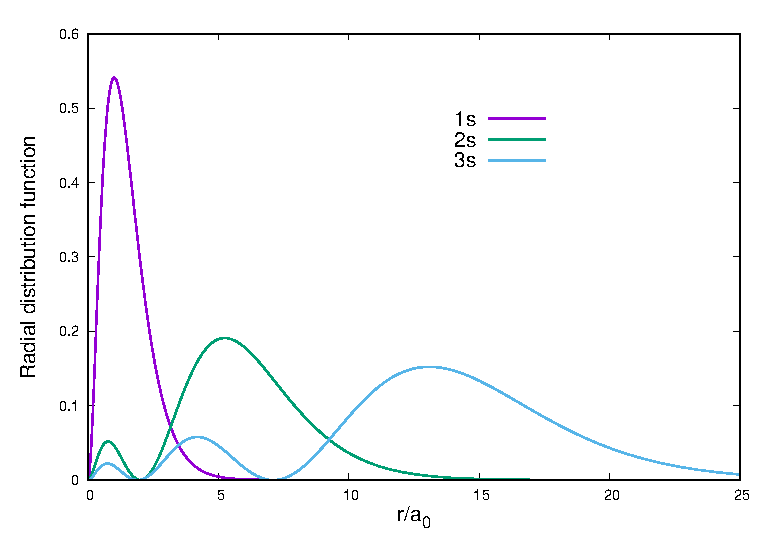
\includegraphics[scale=0.8]{radialdistfuncS.eps}
\caption{Radial distribution function of Hydrogenic 1s, 2s and 3s electron}
\end{figure}
\end{center}
This is the essence of the pseudopotential approximation, the strong core potential is replaced by a pseudopotential, whose ground state wave function resembles the all electron wavefunction outside a selected core radius. In this way both the core states and the wiggles in the valance wavefunctions are removed. For many metals the pseudowavefunctions can be represented by lower number of planewaves. Thus making planewaves a simple and reasonable efficient basis for the pseudo wavefunctions.
\begin{figure}
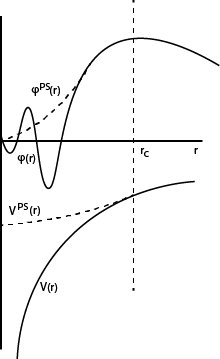
\includegraphics[scale=0.80]{pseudo_figure_01.png}
\caption{Schematic diagram of the replacement of all-electron wave function and core potential by a pseudo-wavefunction and pseudopotential.}
\end{figure}
\subsection{Basic Phillips-Kleinman Construction}
For a given many electron Hamiltonian, $\hat{H}=\hat{T}+\hat{U}$, where $\hat{T}$ is the kinetic energy operator and $\hat{U}$ is the potential energy operator, the core electron wave functions are defined by the \schrod equation
\begin{equation}
 \hat{H}\ket{\psi_i} = \epsilon_i \ket{\psi_i} \quad   (i = 1, n core)
\end{equation}

The valance electron wave function similarly can be found by the Hamiltonian
\begin{equation}
\label{eq_val_hamil}
\hat{H}\ket{\psi_{\upsilon}} = \epsilon_{\upsilon} \ket{\psi_{\upsilon}}
\end{equation}
The valence electron wave function is orthogonal to the core electron wave function ($\braket{\psi_{\upsilon}}{\psi_i}=0$), this orthogonality always has to be preserved, even if the core electrons are not treated explicitly. One way to preserve this orthogonality is to write valence electron wave function in a basis set that is priori orthogonal to the core electrons. The simple Gram-Shmidt orthogonalizatin technique can be used. Using this idea, we can orthogonalize any arbitrary basis set $\{\ket{\chi_n}\}$ to the core electron wave functions by defining a new basis set $\{\ket{\varrho_n}\}$

\begin{equation}
\label{eq_pk}
\ket{\varrho_n} = \ket{\chi_n} - \sum^{ncore}_{i=1} \braket{\psi_i}{\chi_n}\ket{\psi_i}
\end{equation}
Here each of the new basis set, $\{\ket{\varrho_n}\}$, satisfies $\braket{\chi_n}{\psi_i} = 0$ for each $\ket{psi_i}$. Now we can express the valance electron wave function as a linear combination of the new basis sets,
\begin{equation}
\label{eq_val}
\ket{\psi_{\upsilon}} = \sum_n C_n \ket{\varrho_n} 
\end{equation}
Using Eqn~\ref{eq_pk} into the Eqn~\ref{eq_val}, the valence electron can be expressed in the following way. The orthogonality condition with the core electron still valid.
\begin{equation}
\ket{\psi_{\upsilon}} = \sum_n C_n \left [ \ket{\chi_n} - \sum_{i=1}^{ncore} \ket{\psi_i}\braket{\psi_i}{\chi_n} \right ] = \ket{\phi} - \hat{\Omega}\ket{\phi}
\end{equation}
Here, $\hat{\Omega}$ is a projection operator for core electron wave function
\begin{equation}
\label{eq_projection}
\hat{\Omega} = \sum_{i=n}^{ncore} \dyad{\psi_i}{\psi_i}
\end{equation}
and a new wave function which is a linear combination of $\ket{\chi_n}$, sometime designated as pseudo-orbital,
\begin{equation}
\label{eq_pseudoorbital}
\ket{\phi} = \sum_n C_n \ket{\chi_n}
\end{equation}
This technique of representing the valance electron wave function in preorthogonalized basis set has been studied and used as a computational tool~\cite{herring1940new}. It took the insight of the Phillips and Kleinman~\cite{phillips1959new}. The new pseudoorbitals satisfies the orthogonality condition, but it also change the Hamiltonian so that the eigen values are same with the valance electrons. Mathematically, it can be obtained by replacing original valance electron Hamiltonian equation (Eqn~\ref{eq_val_hamil}) with newly obtained pseudo wave function.
\begin{equation}
\label{eq_ps_pot}
\hat{H}\ket{\psi_{\upsilon}} = \hat{H} \left [ \ket{\phi} - \sum_n \ket{\psi_i}\braket{\psi_i}{\phi} \right ] =\epsilon_{\upsilon} \left [ \ket{\phi} - \sum_n \ket{\psi_i}\braket{\psi_i}{\phi}  \right ] 
\end{equation}
Rearranging the above equation provides a new Hamiltonian,
\begin{equation}
\label{eq_ps_hamil}
\left [ \hat{H} + \sum_n ^{ncore} (\epsilon_{\upsilon} - \epsilon_i)\ket{\psi_i}\bra{\psi_i}\right ]\ket{\phi} = 
\epsilon_{\upsilon}\ket{\phi}
\end{equation}
The above equation has the form of the original valance electron eigenequation (\ref{eq_val_hamil}), but with an extra term for preorthogonalization. This extra potential $(V_{nl} = \sum_n^{core} \dyad{\psi_i}{\psi_i})$, is a nonlocal operator, and the pseuodo orbital $(\ket{\phi)}$ is an eigenstate of the new effective Hamiltonian, $\hat{H} + V_{nl}$. The new Hamiltonian has an extra potential $V_{nl}$, which depends on the angular momentum $l$ due to the spherical symmetry. Because of its spherical symmetry, each angular momentum $l$, $m$ can be treated sperately. The dependence on $l$ menas that, a pseudopotential is an non-local operator, can be written in ``semilocal'' (SL) form
\begin{equation}
\label{eq_sl}
\hat{V}_{SL} = \sum_{lm} \ket{Y_{lm}}V_l(r)\bra{Y_{lm}}
\end{equation}
Where $Y_{lm}(\theta,\phi) = P_l(cos(\theta))e^{im\theta}$. It is semilocal because it is non local on the angular variables but local in the radial variable.\footnote{$P_l$ is the Legendre polynomials}


The sophistication and accuracy have evolved considerably since the Phillips-Kleinman construction. This development produces many methods of generating pseudopotentials. All of these methods follow these goals: (1) Pseudopotenal should be as soft as possible, so that it can allow representation of pseudo-wavefunction with fewer planewaves. (2) Transferablity has to be maintained (it means a generated pseudopotential with a configuration should produce other properties accurately) (3) the pseudo-charge density should produce the valance charge density as accurately as possible. Hamann, Schl\"uter and Chiang~\cite{hamann1979norm} developed the concept of norm-coservation, which was a first step to fulfill all the above requirements. Troullier and Martins~\cite{troullier1991efficient} developed a more effective method to generate norm-conserving pseudopotentials for practical calculations.

\subsection{Projector augmented Method: \textit{Mathematical Golem}}
Pseudopotential technique has been proven to be accurate for a large variety of systems, but there is no strict gurantee that it will produce the same results as an all-electron calculation. The challenge with norm-conserving pseudopotentials is that it limits the \textit{softness}. Another way to say it, it needs higher cut-off energy. In the plane-wave basis set for the pseudo wavefunctions is defined by the shortest wave lentgh $\lambda=2\pi/\abs{\vec{G}}$, where $\vec{G}$ is the wave vector. Projector augmented waves (PAW) introduces projectors and auxiliary localized functions to increase the softness of the pseudopotential, at the same time keeping full wave function. In this section I will try to introduce PAW with some basic formalism. The origin of the PAW method lies a transformation that maps the true wavefunctions with their complete nodal structure into auxiliary wavefunctions. The purpose of this transformation is to have a smooth auxiliary wavefunctions, which have a rapidly convergent plane-wave expansion. The PAW method was first proposed by Bl\"ochl in 1994~\cite{blochl1994projector}. The linear transformation is as follows.
\begin{equation}
\ket{\Psi_n} = \hat{\mathcal{T}}\ket{\tilde{\Psi}_n}
\end{equation}
Where, $\ket{\Psi_n}$ is the true all-electron KS single particle wave function, $\ket{\tilde{\Psi}_n}$ is auxiliary smooth wave function, and $\hat{\mathcal{T}}$ is a linear transformation operator. Since the true wave functions are already smooth at a certain minimum distance from the core, $\tilde{\mathcal{T}}$ should only modify the wave function close to the nuclei. Thus the transformation operator becomes
\begin{equation}
\tilde{\mathcal{T}} = 1 + \sum_a \tilde{\mathcal{T}^a}
\end{equation}
Where a is an atom index, $\tilde{\mathcal{T}^a}$, has no effect outside a certain atom-specific augmentation region, $r_C^a$. Inside the augmentation spheres, the true wave function can be expanded in the partial waves $\phi_i^a$, for a corresponding auxiliary smooth partial wave~\footnote{An incoming plane wave along the direction can be expanded in Bessel function. Each angular momentum term is called a partial wave.} can be defined as $\tilde{\phi}_i^a$, and they connected by the following relation.
\begin{equation}
\label{eq_aug_t}
\ket{\phi_i^a} = (1+\hat{\mathcal{T}}^a)\ket{\tilde{\phi}_i^a} \Rightarrow  \hat{\mathcal{T}}^a \ket{\phi_i^a} = \ket{\phi_i^a} - \ket{\tilde{\phi}_i^a}
\end{equation} 
Here $a$ is an atom index, $i$ comes from partial waves. Outside the augmentation sphere, the partial wave and its smooth counterpart should be identical.
\begin{equation}
\phi_i^a(\mathbf{r}) = \tilde{\phi}_i^a(\mathbf{r}),\  for \quad r > r_c^a
\end{equation} 
Where $\phi_i^a(\mathbf{r})=\braket{\mathbf{r}}{\phi_i^a}$, and similar for $\tilde{\phi}_i^a$. If the smooth partial waves form a complete set inside the augmentation sphere, we can expand the smooth all electron wave functions as 
\begin{equation}
\ket{\tilde{\Psi}_i^a} = \sum_i P_{ni}^a \ket{\tilde{\phi}_i^a}, \quad \abs{\mathbf{r}-\mathbf{R}} < r_c^a
\end{equation}
Where, $P_{na}^a$ are expansion coefficients, and need to be determined. And also, the index a stands for atomic sites, i to dintinguish different partials waves and n connected to quantum numbers $(l,m)$. Since the transformation operator connects the smooth pseudo wave function to true wave function.
\begin{equation}
\ket{\Psi_n} = \hat{\mathcal{T}} \ket{\tilde{\Psi}_n} = \sum_i P_{ni}^a \ket{\psi_i^a}, \quad \abs{\mathbf{r}-\mathbf{R}} < r_c^a
\end{equation} 
Something really interesting about the above equation, the true wave function has the same expansion coefficient $(P_{ni}^a)$ as the pseudo wavefucntion. The transformation operator $\hat{\mathcal{T}}$ is required to be linear, the coefficient must be linear functionals of $\ket{\tilde{\Psi}_n}$, i.e.
\begin{equation}
P_{ni}^a = \braket{\tilde{p}_i^a}{\tilde{\Psi}_n}
\end{equation}
Where $\ket{\tilde{p}_i^a}$ are some fixed functions termed smooth projector functions. As there is no overlap between the augmentation spheres, we expect the smooth all electron wave function, $\ket{\tilde{\Psi}_n^a} = \sum_i \ket{\tilde{\phi}_i^a} \braket{\tilde{p}_i^a}{\tilde{\Psi}_n}$. The projectors have to be localized within an augmentation region
\begin{equation}
\label{eq_paw_complete}
	\sum_i \dyad{\tilde{\phi}_i^a}{\tilde{p}_i^a} = 1
\end{equation}
This also implied that
\begin{equation}
	\braket{\tilde{p}_{i_1}^a}{\tilde{\phi}_{i_2}^a} = \delta_{i_1,i_2},\quad for \quad < r_c^a
\end{equation}
the projector functions should be orthonormal to the smooth partial waves inside the augmentation sphere. The choice of projectors and partial waves can be found more detailed form original work of Bl\"ochl~\cite{blochl1994projector}. Using the completeness relation from Eqn~\ref{eq_paw_complete}
\begin{equation}
\hat{\mathcal{T}^a} = \sum_i \hat{\mathcal{T}^a} \dyad{\tilde{\phi}_i^a}{\tilde{p}_i^a} = \sum_i \left( \ket{\phi_i^a} -\ket{\tilde{\phi}_i^a} \right) \bra{\tilde{p}_i^a}
\end{equation}
Remember, the operator $\hat{\mathcal{T}}^a$ operates only inside the sphere, outside sphere it behave like this $\ket{\phi_i^a} - \ket{\tilde{\phi}_i^a}$. Thus the total transformation operator becomes
\begin{equation}
\hat{\mathcal{T}} = 1 + \sum_a\sum_i\left( \ket{\phi_i^a} -\ket{\tilde{\phi}_i^a} \right) \bra{\tilde{p}_i^a} 
\end{equation}
To summarize, we obtain the all electron KS wave function $\ket{\Psi_n(\mathbf{r})} = \braket{\mathbf{r}}{\Psi_n}$ from the transformation
\begin{equation}
\label{eq_main_paw}
\Psi_n(\mathbf{r}) = \tilde{\Psi}_n(\mathbf{r}) + \sum_a\sum_i \left (\phi_i^a(\mathbf{r}) - \tilde{\phi}_i^a(\mathbf{r})   \right) \braket{\tilde{p}_i^a}{\tilde{\psi}_n}
\end{equation}
The equation above has three different components in the right. The first is the auxiliary wave function. The second term is the sum of partial waves, the last term is the sum of pseudo partial waves that must be subtracted inside the augmentation region. To make it a simple KS wave function representation
\begin{equation}
\psi_n(\mathbf{r}) = \tilde{\psi}_n(\mathbf{r}) + \sum_a\left( \psi_n^a(\mathbf{r}-\mathbf{R}^a) - \tilde{\psi}_n^a (\mathbf{r} - \mathbf{R}^a) \right)
\end{equation}

The trouble of the original KS wave functions, was that they display rapid oscillations in some of the space and smooth behavior in other parts of space. By decomposing the wave function, the achievement is that the original wave function is separated into auxiliary wave functions which are smooth everywhere.

